% This template has been tested with IEEEtran of 2015.
% Template from https://github.com/latextemplates/IEEE

% !TeX spellcheck = en-US
% !TeX encoding = utf8
% !TeX program = pdflatex
% !BIB program = bibtex
% -*- coding:utf-8 mod:LaTeX -*-

% To set up:
% aptitude install texlive-publishers texlive-lang-european texlive-latex-extra

% PBROWN: Use this to suppress the warning when including multiple matplotlib PDF plots on the same page
\pdfsuppresswarningpagegroup=1

%cmap has to be loaded before any font package (such as newtxmath)
\RequirePackage{cmap}

% DO NOT DOWNLOAD IEEEtran.cls - Use the one of your LaTeX distribution
% On Ubuntu, aptitude install texlive-publishers
\documentclass[conference,a4paper]{IEEEtran}[2015/08/26]

% use nicer font for code
\usepackage[zerostyle=b,scaled=.75]{newtxtt}

\usepackage[T1]{fontenc}
\usepackage[utf8]{inputenc} %support umlauts in the input
% I added the following to get Times Roman in math. Otherwise the g's looked really different.
% See https://tex.stackexchange.com/questions/9685/math-and-times-font#9686
\usepackage[italic]{mathastext}

\usepackage{graphicx}

%\usepackage[inkscapelatex=false]{svg}

%Set English as language and allow to write hyphenated"=words
% For Turkish, on Ubuntu aptitude install texlive-lang-european
%\usepackage[english]{babel}
% If using Turkish, also set option shorthands=off
%Hint by http://tex.stackexchange.com/a/321066/9075 -> enable "= as dashes
%\addto\extrasenglish{\languageshorthands{ngerman}\useshorthands{"}}

% backticks (`) are rendered as such in verbatim environment. See https://tex.stackexchange.com/a/341057/9075 for details.
\usepackage{upquote}

%extended enumerate, such as \begin{compactenum}
\usepackage{paralist}

%for easy quotations: \enquote{text}
\usepackage{csquotes}

\usepackage{amsmath}

%enable margin kerning
\RequirePackage{iftex}
\ifPDFTeX
  \RequirePackage[%
    final,%
    expansion=alltext,%
    protrusion=alltext-nott]{microtype}%
\else
  \RequirePackage[%
    final,%
    protrusion=alltext-nott]{microtype}%
\fi%
% \texttt{test -- test} keeps the "--" as "--" (and does not convert it to an en dash)
\DisableLigatures{encoding = T1, family = tt* }

%tweak \url{...}
\usepackage{url}
%\urlstyle{same}
%improve wrapping of URLs - hint by http://tex.stackexchange.com/a/10419/9075
\makeatletter
\g@addto@macro{\UrlBreaks}{\UrlOrds}
\makeatother
%nicer // - solution by http://tex.stackexchange.com/a/98470/9075
%DO NOT ACTIVATE -> prevents line breaks
%\makeatletter
%\def\Url@twoslashes{\mathchar`\/\@ifnextchar/{\kern-.2em}{}}
%\g@addto@macro\UrlSpecials{\do\/{\Url@twoslashes}}
%\makeatother

% Diagonal lines in a table - http://tex.stackexchange.com/questions/17745/diagonal-lines-in-table-cell
% Slashbox is not available in texlive (due to licensing) and also gives bad results. This, we use diagbox
%\usepackage{diagbox}

\usepackage{booktabs}

% Required for package pdfcomment later
\usepackage{xcolor}

% For listings
\usepackage{listings}
\lstset{%
  basicstyle=\ttfamily,%
  columns=fixed,%
  basewidth=.5em,%
  xleftmargin=0.5cm,%
  captionpos=b}%

% Enable nice comments
\usepackage{pdfcomment}
%
\newcommand{\commentontext}[2]{\colorbox{yellow!60}{#1}\pdfcomment[color={0.234 0.867 0.211},hoffset=-6pt,voffset=10pt,opacity=0.5]{#2}}
\newcommand{\commentatside}[1]{\pdfcomment[color={0.045 0.278 0.643},icon=Note]{#1}}
%
% Compatibility with packages todo, easy-todo, todonotes
\newcommand{\todo}[1]{\commentatside{#1}}
% Compatiblity with package fixmetodonotes
\newcommand{\TODO}[1]{\commentatside{#1}}

% Bibliopgraphy enhancements
%  - enable \cite[prenote][]{ref}
%  - enable \cite{ref1,ref2}
% Alternative: \usepackage{cite}, which enables \cite{ref1, ref2} only (otherwise: Error message: "White space in argument")
%
% Doc: http://texdoc.net/natbib

% normal IEEE
%\usepackage[%
%	square,        % for square brackets
%	comma,         % use commas as separators
%	numbers,       % for numerical citations;
%	%sort           % orders multiple citations into the sequence in which they appear in the list of references;
%	sort&compress % as sort but in addition multiple numerical citations
%	               % are compressed if possible (as 3-6, 15);
%]{natbib}
% Same fontsize as without natbib
%\renewcommand{\bibfont}{\normalfont\footnotesize}
% Using cite package instead
\usepackage{cite}

% Enable hyperlinked author names in the case of \citet
% Source: https://tex.stackexchange.com/a/76075/9075
\usepackage{etoolbox}
\makeatletter
\patchcmd{\NAT@test}{\else \NAT@nm}{\else \NAT@hyper@{\NAT@nm}}{}{}
\makeatother

% Enable that parameters of \cref{}, \ref{}, \cite{}, ... are linked so that a reader can click on the number an jump to the target in the document
\usepackage{hyperref}
% Enable hyperref without colors and without bookmarks
\hypersetup{hidelinks,
  colorlinks=true,
  allcolors=black,
  pdfstartview=Fit,
  breaklinks=true}
%
% Enable correct jumping to figures when referencing
\usepackage[all]{hypcap}

%\renewcommand{\figurename}{Fig.}

%enable \cref{...} and \Cref{...} instead of \ref: Type of reference included in the link
\usepackage[capitalise,nameinlink]{cleveref}
%\crefname{lstlisting}{\lstlistingname}{\lstlistingname}
%\Crefname{lstlisting}{Listing}{Listings}
% The following are to comply with the IEEE style guide.
\crefformat{equation}{#2(#1)#3}
\Crefformat{equation}{#2Equation (#1)#3}
\crefname{figure}{Fig.}{Figs.}
%\Crefname{figure}{Fig.}{Figs.}

%Following definitions are outside of IfPackageLoaded; inside, they are not visible
%
%Intermediate solution for hyperlinked refs. See https://tex.stackexchange.com/q/132420/9075 for more information.
\newcommand{\Vlabel}[1]{\label[line]{#1}\hypertarget{#1}{}}
\newcommand{\lref}[1]{\hyperlink{#1}{\FancyVerbLineautorefname~\ref*{#1}}}

\newenvironment{listing}[1][htbp!]{\begin{figure}[#1]}{\end{figure}}
\newcounter{listing}

\usepackage{xspace}
%\newcommand{\eg}{e.\,g.\xspace}
%\newcommand{\ie}{i.\,e.\xspace}
\newcommand{\eg}{e.\,g.,\ }
\newcommand{\ie}{i.\,e.,\ }

%introduce \powerset - hint by http://matheplanet.com/matheplanet/nuke/html/viewtopic.php?topic=136492&post_id=997377
\DeclareFontFamily{U}{MnSymbolC}{}
\DeclareSymbolFont{MnSyC}{U}{MnSymbolC}{m}{n}
\DeclareFontShape{U}{MnSymbolC}{m}{n}{
  <-6>    MnSymbolC5
  <6-7>   MnSymbolC6
  <7-8>   MnSymbolC7
  <8-9>   MnSymbolC8
  <9-10>  MnSymbolC9
  <10-12> MnSymbolC10
  <12->   MnSymbolC12%
}{}
\DeclareMathSymbol{\powerset}{\mathord}{MnSyC}{180}

% *** SUBFIGURE PACKAGES ***
\ifCLASSOPTIONcompsoc
  \usepackage[caption=false,font=footnotesize,labelfont=sf,textfont=sf]{subfig}
\else
  \usepackage[caption=false,font=footnotesize]{subfig}
\fi

\usepackage{stfloats}



% correct bad hyphenation here
\hyphenation{op-tical net-works semi-conduc-tor}

\graphicspath{{./figs/}}

% Paper-specific packages that I have added:
\usepackage{siunitx}  % For units with \SI
\usepackage{threeparttable}  % For tablenotes
\usepackage{placeins}  % For \FloatBarrier
\usepackage{xfrac}  % For \sfrac
%\usepackage{orcidlink}  % For orcid link
\DeclareMathOperator{\logicand}{and}
\DeclareMathOperator{\logicor}{or}


%\bibliographystyle{chicago}   % For drafts only, to make it easier to see which references have been used.
\bibliographystyle{IEEEtran} % IEEEtranN is the natbib compatible bst file
%\usepackage{showkeys}          % For drafts only


\begin{document}
%\IEEEoverridecommandlockouts
\bstctlcite{IEEEexample:BSTcontrol}

\title{Lightweight Photovoltaic Forecasting Method for Agricultural Microgrids}

\author{%
  \IEEEauthorblockN{Paul D. Brown}%\textsuperscript{\orcidlink{0000-0001-5753-0449}}}%
  \IEEEauthorblockA{Department of Electrical and Electronics Engineering\\
  	Middle East Technical University\\
  	Ankara, Turkey\\
  	ORCID: 0000-0001-5753-0449}
\and
  \IEEEauthorblockN{Murat Göl}%\textsuperscript{\orcidlink{0000-0002-2523-1169}}}%
  %\orcidlink{0000-0001-5753-0449}
  \IEEEauthorblockA{Department of Electrical and Electronics Engineering\\
    Middle East Technical University\\
	Ankara, Turkey\\
	ORCID: 0000-0002-2523-1169}
}

% No paper headers for conference
%\markboth{ISGT Europe, October 2023}%
%{{Brown}: Lightweight Photovoltaic Forecasting Method for Agricultural Microgrid}

% use for special paper notices
%\IEEEspecialpapernotice{(Invited Paper)}

% make the title area
\maketitle

% In case you want to add a copyright statement.
%
% Source: https://tex.stackexchange.com/a/200330/9075
%
% All possible solutions:
%  - https://tex.stackexchange.com/a/325013/9075
%  - https://tex.stackexchange.com/a/279134/9075
%  - https://tex.stackexchange.com/q/279789/9075 (TikZ)
%  - https://tex.stackexchange.com/a/200330/9075 - for non-compsocc papers
\iffalse
    \makeatletter
    \def\ps@IEEEtitlepagestyle{%
      \def\@oddfoot{\mycopyrightnotice}%
      \def\@evenfoot{}%
    }
    \makeatother
    \def\mycopyrightnotice{%
      \begin{minipage}{\textwidth}
        \footnotesize
        979-8-3503-9678-2/23/\$31.00 ©2023 IEEE
      \end{minipage}
      \gdef\mycopyrightnotice{}% just in case
    }
\fi

\begin{abstract}
  % Abstract_should_be_150_to_200_words.
A lightweight forecasting method was developed for day-ahead (12 to 72-hours) and intra-day forecasting of photovoltaic (PV) array power output for use with energy management of agricultural microgrids.
The proposed method allows the PV output to be forecast without requiring extensive computing resources or high-bandwidth communication channel to the PV site.
The proposed day-ahead forecasting method combines historical PV output data with historical weather data to infer the relationship between weather and PV output by fitting a simple regression model.
Based on the assumption that updated weather forecasts are in general not obtained throughout the day, the current-day PV output forecast was updated using time-series techniques.
The proposed forecasting methods were applied to a dataset of rooftop PV output
and compared to reference persistence forecasts.
The method was demonstrated by using the forecasts in the optimized operation of an agricultural microgrid
and simulating with actual PV output.
\end{abstract}

\begin{IEEEkeywords}
	Photovoltaic systems, forecasting, agriculture
\end{IEEEkeywords}

% For peer review papers, you can put extra information on the cover
% page as needed:
% \ifCLASSOPTIONpeerreview
% \begin{center} \bfseries EDICS Category: 3-BBND \end{center}
% \fi
%
% For peerreview papers, this IEEEtran command inserts a page break and
% creates the second title. It will be ignored for other modes.
\IEEEpeerreviewmaketitle

\section{Introduction}
\label{sec:intro}

Over recent decades, many factors have driven significant changes in the electrical power industry,
including climate change,
the growing use of renewable energy resources,
and ongoing rural electrification.
For agricultural consumers, electrification enables increased yields and economic development.
Ref. \cite{Mandelli2016} reviews technology and applications for off-grid systems for rural electrification.

For agricultural applications, photovoltaic (PV) energy is generally well aligned with water needs\cite{Aliyu2018}.
Ref. \cite{Aliyu2018} reviews numerous solar-powered water pumping applications around the world while \cite{Muhsen2017} reviews the PV and water pumping modeling, design, and control approaches in the literature.

One of the barriers to efficient use of PV energy in the grid and in micro-grids
is the difficulty of accurately predicting future energy availability.
As reviewed in \cite{Antonanzas2016}, many techniques have been developed for forecasting PV energy over various time horizons.
The authors of this paper have been working on techniques for optimal energy planning for agricultural microgrids.
For operational optimization, an effective day-ahead PV forecasting method was needed.
In recent years, LSTM-based neural networks have emerged as the state-of-the art
for day-ahead PV energy forecasting
\cite{Kuo2022,Aslam2021,Liu2021}.

As promising as deep learning networks are for day-ahead forecasting,
they have the drawback of requiring 
a lot of historical data\cite{Aillaud2020} and significant computational resources for training.
Agricultural microgrids, on the other hand, are often implemented in locations where communication infrastructure is weak
and bandwidth and/or availability are limited.
To cope with these conditions, the authors developed methods for day-ahead PV forecasting with a design goal to be ``lightweight'', that is to require minimal weather forecast data, site-specific modeling data, historical generation data, and computational resources.
The target computing platform for the developed method is a single-board computer such as the Raspberry Pi or similar.


% Make sure any figures start AFTER the introduction and don't float above it.
\FloatBarrier

The literature survey will be part of the introduction.







\section{Proposed Method}
\label{sec:proposed-method}

The proposed method utilizes meteorological forecast data such as forecast cloudiness or forecast irradiance to forecast the PV system output for the upcoming 12 to 72 hours, which called the ``day-ahead forecast''.
It is assumed that these meteorological forecasts will be updated once or at most a few times per day.
Throughout the day, the current day's PV output forecast is updated by applying one of several available time-series forecasting techniques.
A high-level diagram of the proposed forecast method is shown in \cref{fig:PV_forecast_flowchart}.

\begin{figure}[t]
	\centering
	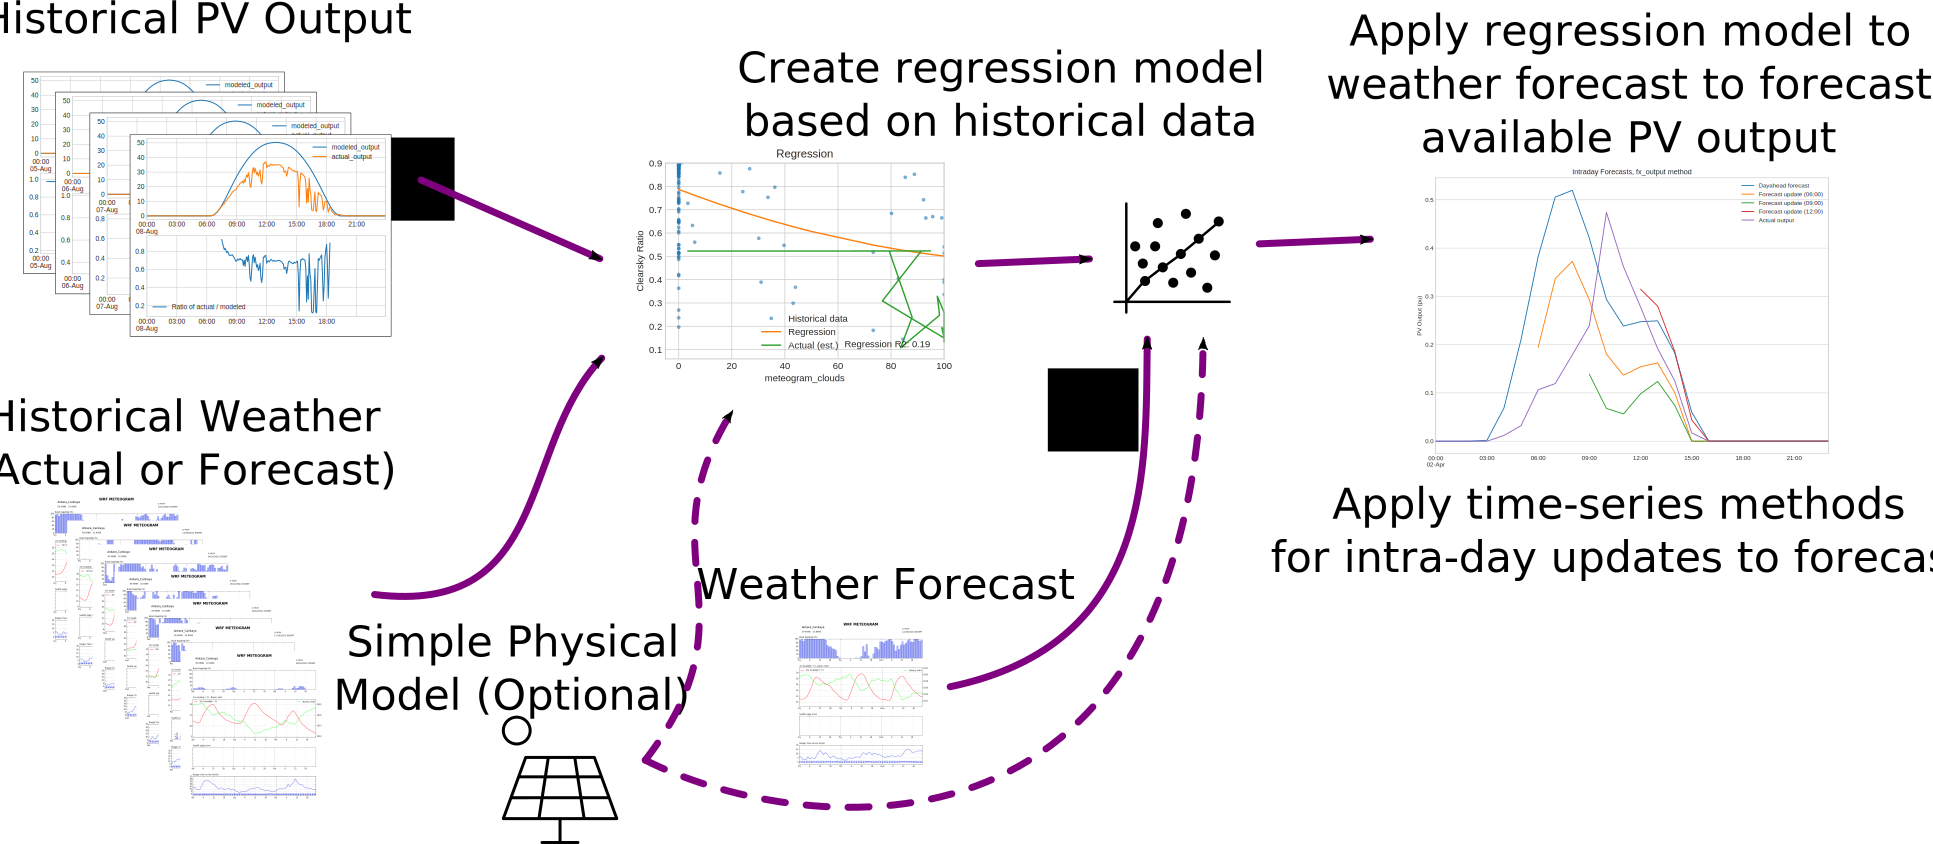
\includegraphics[width=1.0\columnwidth]{PV_forecast_flowchart}
	\caption{Flowchart of Forecasting Method}
	\label{fig:PV_forecast_flowchart}
\end{figure}


\subsection{Day-Ahead Forecasts}
\label{sec:method-day-ahead}

The proposed day-ahead forecasting method combines historical PV output data with historical weather data to infer the relationship between weather and PV output by fitting a simple regression model.

Some pre-processing of the historical data was done prior to  fitting the regression model.
Data from periods of darkness, when output goes to small or negative values, were removed.
This also removed periods when the PV array was covered with snow.

How the regression model was applied depends on the weather data that was used.
If the weather data used represented the incoming solar energy, then the regression was done directly between the weather data and PV output.
Weather data utilized of this type was the global horizontal irradiance (ghi).

On the other hand, weather data that represented the attenuation of incoming solar energy was regressed against the clear-sky ratio for PV output.
Two methods were developed for calculating the clear-sky ratio.
The first method was to roughly model the PV array using data for its geographic position and orientation to obtain modeled clear-sky output.
The second method was to estimate the maximum possible output at each time of day by calculating the maximum observed PV output for each time of day in the historical data window.
This second method had the advantage of not requiring any modeling information about the PV array.
It had the further advantage of naturally incorporating effects of shading of the array during parts of the day due to obstructions.
Since the data set used for this analysis did not include any shading of the array, this last benefit could not be assessed in comparison to other methods.

The formula used to calculate the clear-sky ratio is shown in \cref{eqn:clear-sky-ratio},
where $r_{cs}$ is the clear-sky ratio, $P_{out}$ is the PV output, and $P_{cs}$ is the clear-sky PV output.
In order to provide numerical stability of the clear-sky ratio for periods when the clear-sky output is small, the parameters $\epsilon$ and $r_\epsilon$ were incorporated so that as $P_{cs}$ goes to zero, the clear-sky ratio $r_{cs}$ will approach $r_\epsilon$.

\begin{equation}
	\label{eqn:clear-sky-ratio}
	r_{cs} = \frac{P_{out} + r_\epsilon \epsilon}{P_{cs} + \epsilon}
\end{equation}

The regression model was then fit to the transformed data.
A second-degree polynomial model was used in the case of ghi weather forecasts as well as the case of cloudiness weather forecasts.
The fit model was then applied to the weather forecast data available for the forecast period.
If applicable, the resulting forecast was then converted from a forecast clear-sky ratio back to PV output.

\subsection{Intra-day Updates}
\label{sec:method-intraday}

Based on the assumption that updated weather forecasts are in general not obtained throughout the day, the current-day PV output forecast was updated using time-series techniques. Several approaches to intra-day updates were investigated as described in the following paragraphs.

\textit{AR(2) on actual output with exogenous variable:}
An auto-regressive time series model with two lags was applied to the actual clear-sky output ratio with the day-ahead clear-sky output forecast included in the model as an exogenous variable.

\textit{SARIMAX:}
A seasonal auto-regressive integrated moving average model was applied to the actual PV power output with day-ahead output power forecast included in the model as an exogenous variable.
This model is characterized by parameters for the number of lags, order of differencing, and order of the moving average, for both the trend and seasonal components.
A variety of parameter combinations was tested against the data, and the best performing model was with AR(1) and MA(2), with the day-ahead PV output power forecast as an exogenous variable, and with no differencing or seasonal components included.

\textit{AR(2) on residual of PV output:}
An auto-regressive time series model with two lags was applied to the residual between actual PV output and the day-ahead forecast PV output. The forecast output of the model was then added as a correction term to the day-ahead PV output forecast for the intra-day period.

\textit{AR(2) on residual of clear-sky ratio:}
An auto-regressive time series model with two lags was applied to the residual between the actual clear-sky ratio and the day-ahead forecast clear-sky ratio. The forecast output of the model was then added as a correction term to the day-ahead clear-sky ratio forecast for the intra-day period.

\textit{Scaling:}
The day-ahead forecast for the rest of the day was scaled using the ratio between the actual output in the previous period and the day-ahead forecast for the previous period.



\section{Data Sources}
\label{sec:data-source}

The PV time series used for this analysis was the recorded output power of the rooftop PV array on the METU EEE Department machinery building in Ankara, Turkey.
Recordings were obtained by downloading them from the logger integrated with the inverter for the PV array.
Logged data was recorded at approximately five-minute intervals.
For the forecasting method, the logged data was aligned to exact five-minute intervals even with the hour using linear interpolation and then aggregated to hourly intervals by the mean.
For the operational model, these values were scaled to the rating of the demonstration system.


The weather forecast data used for this analysis was obtained from multiple sources.
Firstly, WRF Meteogram forecasts have been saved from the Turkish Meteorology Directorate (MGM)\cite{MGM_Meteogram}.
Since the MGM meteograms are available as a image rather than as structured data, code was developed to extract data from the plots in the meteogram and output it in csv format\cite{MeteogramExtractGithubRepo}.
Secondly, forecasts were obtained from the SolCast PV-focused weather service\cite{Solcast}.
SolCast weather forecasts include both a cloudiness forecast as well as an irradiance (ghi) forecast along with many other forecast quantities.
SolCast data is provided using an API, so no special data extraction or conversion was needed.

% OpenWeather weather service\cite{OpenWeather} was downloaded but currently is not being used.

\section{Implementation}
\label{sec:implementation}

The forecasting code was implemented using the Python programming language\cite{Python3}.
The Pandas\cite{Pandas} data analysis library and NumPy\cite{NumPy} were used for data manipulation.
Scikit-learn\cite{scikit-learn} was used for fitting the regression model and generating predictions from it.
Statsmodels\cite{statsmodels} was used for fitting time-series auto-regressive models and generating predictions.
Plots were generated using Matplotlib\cite{Matplotlib}.
The optimization and simulation implementation was previously described in \cite{Brown2022}.
Full implementation details can be obtained by examining the source code released on GitHub\cite{ELECO2023GithubRepo} and CodeOcean\cite{ELECO2023CodeOceanRepo}.

\section{Results}
\label{sec:results}

Results will be presented in this section. Plots! Tables! Yay!




\section{Conclusion}
\label{sec:conclusion}

This is the conclusion section. It should be all new and focus on the additional forecasting work to do.

%\clearpage

% use section* for acknowledgment
\ifCLASSOPTIONcompsoc
  % The Computer Society usually uses the plural form
  %\section*{Acknowledgments}
\else
  % regular IEEE prefers the singular form
  \section*{Acknowledgment}
  This work is supported by the Scientific and Technological
  Research Council of Turkey (TUBITAK) under grant number
  119N313.
\fi

% The Acknowledgment section is commented out.

% trigger a \newpage just before the given reference
% number - used to balance the columns on the last page
% adjust value as needed - may need to be readjusted if
% the document is modified later
%\IEEEtriggeratref{8}
% The "triggered" command can be changed if desired:
%\IEEEtriggercmd{\enlargethispage{-5in}}

% Enable to reduce spacing between bibitems (source: https://tex.stackexchange.com/a/25774)
% \def\IEEEbibitemsep{0pt plus .5pt}

% argument is your BibTeX string definitions and bibliography database(s)
\bibliography{IEEEabrv,biblio}
% Manually include bibliography for the final version
%% !TeX spellcheck = en-US
% !TeX encoding = utf8
% !TeX program = pdflatex
% !BIB program = bibtex
% -*- coding:utf-8 mod:LaTeX -*-

% To set up:
% aptitude install texlive-publishers texlive-lang-european texlive-latex-extra

% PBROWN: Use this to suppress the warning when including multiple matplotlib PDF plots on the same page
\pdfsuppresswarningpagegroup=1

\RequirePackage{fix-cm}

%cmap has to be loaded before any font package (such as newtxmath)
\RequirePackage{cmap}

% Found eleco2013 code in ELECO 2017 conference archive

\documentclass[9pt]{extarticle}
\usepackage{eleco}

\usepackage{orcidlink}

\usepackage[T1]{fontenc}
\usepackage[utf8]{inputenc} %support umlauts in the input

\usepackage{graphicx}

%\usepackage[inkscapelatex=false]{svg}

%Set English as language and allow to write hyphenated"=words
% For Turkish, on Ubuntu aptitude install texlive-lang-european
%\usepackage[english]{babel}
% If using Turkish, also set option shorthands=off
%Hint by http://tex.stackexchange.com/a/321066/9075 -> enable "= as dashes
%\addto\extrasenglish{\languageshorthands{ngerman}\useshorthands{"}}

% backticks (`) are rendered as such in verbatim environment. See https://tex.stackexchange.com/a/341057/9075 for details.
%\usepackage{upquote}

%for easy quotations: \enquote{text}
\usepackage{csquotes}

%enable margin kerning
\RequirePackage{iftex}
\ifPDFTeX
  \RequirePackage[%
    final,%
    expansion=alltext,%
    protrusion=alltext-nott]{microtype}%
\else
  \RequirePackage[%
    final,%
    protrusion=alltext-nott]{microtype}%
\fi%
% \texttt{test -- test} keeps the "--" as "--" (and does not convert it to an en dash)
%\DisableLigatures{encoding = T1, family = tt* }

%tweak \url{...}
\usepackage{url}
%\urlstyle{same}
%improve wrapping of URLs - hint by http://tex.stackexchange.com/a/10419/9075
\makeatletter
\g@addto@macro{\UrlBreaks}{\UrlOrds}
\makeatother
%nicer // - solution by http://tex.stackexchange.com/a/98470/9075
%DO NOT ACTIVATE -> prevents line breaks
%\makeatletter
%\def\Url@twoslashes{\mathchar`\/\@ifnextchar/{\kern-.2em}{}}
%\g@addto@macro\UrlSpecials{\do\/{\Url@twoslashes}}
%\makeatother

% Diagonal lines in a table - http://tex.stackexchange.com/questions/17745/diagonal-lines-in-table-cell
% Slashbox is not available in texlive (due to licensing) and also gives bad results. This, we use diagbox
%\usepackage{diagbox}

\usepackage{booktabs}
\usepackage{multirow}  % If needed for any  multi-row table cells

% Required for package pdfcomment later
\usepackage{xcolor}

% For listings
%\usepackage{listings}
%\lstset{%
%  basicstyle=\ttfamily,%
%  columns=fixed,%
%  basewidth=.5em,%
%  xleftmargin=0.5cm,%
%  captionpos=b}%

% Enable nice comments
\usepackage[final]{pdfcomment}
%
% color={0.045 0.278 0.643}  % Blue
% color={0.234 0.867 0.211 % Light green
\newcommand{\commentontext}[2]{\colorbox{yellow!60}{#1}\pdfcomment[color={0.234 0.867 0.211},hoffset=-6pt,voffset=10pt,opacity=0.5]{#2}}
\newcommand{\commentatside}[1]{\pdfcomment[color=yellow,icon=Note]{#1}}
%
% Compatibility with packages todo, easy-todo, todonotes
\newcommand{\todo}[1]{\commentatside{#1}}
% Compatiblity with package fixmetodonotes
\newcommand{\TODO}[1]{\commentatside{#1}}

% Bibliography enhancements
%  - enable \cite[prenote][]{ref}
%  - enable \cite{ref1,ref2}
% Alternative: \usepackage{cite}, which enables \cite{ref1, ref2} only (otherwise: Error message: "White space in argument")
%
% Doc: http://texdoc.net/natbib

% normal IEEE
%\usepackage[%
%	square,        % for square brackets
%	comma,         % use commas as separators
%	numbers,       % for numerical citations;
%	%sort           % orders multiple citations into the sequence in which they appear in the list of references;
%	sort&compress % as sort but in addition multiple numerical citations
%	               % are compressed if possible (as 3-6, 15);
%]{natbib}
% Same fontsize as without natbib
%\renewcommand{\bibfont}{\normalfont\footnotesize}
% Using cite package instead
\usepackage{cite}

% Enable hyperlinked author names in the case of \citet
% Source: https://tex.stackexchange.com/a/76075/9075
%\usepackage{etoolbox}
%\makeatletter
%\patchcmd{\NAT@test}{\else \NAT@nm}{\else \NAT@hyper@{\NAT@nm}}{}{}
%\makeatother

% Enable that parameters of \cref{}, \ref{}, \cite{}, ... are linked so that a reader can click on the number an jump to the target in the document
\usepackage{hyperref}
% Enable hyperref without colors and without bookmarks
\hypersetup{hidelinks,
  colorlinks=true,
  allcolors=black,
  pdfstartview=Fit,
  breaklinks=true}
%
% Enable correct jumping to figures when referencing
\usepackage[all]{hypcap}

%\renewcommand{\figurename}{Fig.}

%enable \cref{...} and \Cref{...} instead of \ref: Type of reference included in the link
\usepackage[capitalise,nameinlink]{cleveref}
% The following are to comply with the IEEE style guide.
\crefformat{equation}{#2(#1)#3}
\Crefformat{equation}{#2Equation (#1)#3}
\crefname{figure}{Fig.}{Figs.}

%Following definitions are outside of IfPackageLoaded; inside, they are not visible
%
%Intermediate solution for hyperlinked refs. See https://tex.stackexchange.com/q/132420/9075 for more information.
%\newcommand{\Vlabel}[1]{\label[line]{#1}\hypertarget{#1}{}}
%\newcommand{\lref}[1]{\hyperlink{#1}{\FancyVerbLineautorefname~\ref*{#1}}}
%
%\newenvironment{listing}[1][htbp!]{\begin{figure}[#1]}{\end{figure}}
%\newcounter{listing}

%\usepackage{xspace}
%\newcommand{\eg}{e.\,g.\xspace}
%\newcommand{\ie}{i.\,e.\xspace}
\newcommand{\eg}{e.\,g.,\ }
\newcommand{\ie}{i.\,e.,\ }

%%introduce \powerset - hint by http://matheplanet.com/matheplanet/nuke/html/viewtopic.php?topic=136492&post_id=997377
%\DeclareFontFamily{U}{MnSymbolC}{}
%\DeclareSymbolFont{MnSyC}{U}{MnSymbolC}{m}{n}
%\DeclareFontShape{U}{MnSymbolC}{m}{n}{
%  <-6>    MnSymbolC5
%  <6-7>   MnSymbolC6
%  <7-8>   MnSymbolC7
%  <8-9>   MnSymbolC8
%  <9-10>  MnSymbolC9
%  <10-12> MnSymbolC10
%  <12->   MnSymbolC12%
%}{}
%\DeclareMathSymbol{\powerset}{\mathord}{MnSyC}{180}

% *** SUBFIGURE PACKAGES ***
%\usepackage[caption=false,font=footnotesize]{subfig}

%\usepackage{stfloats}



% correct bad hyphenation here
\hyphenation{op-tical net-works semi-conduc-tor}

\graphicspath{{./figs/}}

% Paper-specific packages that I have added:
\usepackage{siunitx}  % For units with \SI
\usepackage{threeparttable}  % For tablenotes
\usepackage{placeins}  % For \FloatBarrier
\usepackage{xfrac}  % For \sfrac
%\usepackage{orcidlink}  % For orcid link
\DeclareMathOperator{\logicand}{and}
\DeclareMathOperator{\logicor}{or}


%\bibliographystyle{chicago}   % For drafts only, to make it easier to see which references have been used.
%\bibliographystyle{IEEEtran} % IEEEtranN is the natbib compatible bst file
%\usepackage{showkeys}          % For drafts only


\begin{document}
%\IEEEoverridecommandlockouts
\bstctlcite{IEEEexample:BSTcontrol}

\title{Lightweight Photovoltaic Forecasting Method for Agricultural Microgrids}

\author{%
  \IEEEauthorblockN{Paul D. Brown}%\textsuperscript{\orcidlink{0000-0001-5753-0449}}}%
  \IEEEauthorblockA{Department of Electrical and Electronics Engineering\\
  	Middle East Technical University\\
  	Ankara, Turkey\\
  	ORCID: 0000-0001-5753-0449}
\and
  \IEEEauthorblockN{Murat Göl}%\textsuperscript{\orcidlink{0000-0002-2523-1169}}}%
  %\orcidlink{0000-0001-5753-0449}
  \IEEEauthorblockA{Department of Electrical and Electronics Engineering\\
    Middle East Technical University\\
	Ankara, Turkey\\
	ORCID: 0000-0002-2523-1169}
}

% No paper headers for conference
%\markboth{ISGT Europe, October 2023}%
%{{Brown}: Lightweight Photovoltaic Forecasting Method for Agricultural Microgrid}

% make the title area
\maketitle
\begin{abstract}
  % Abstract_should_be_150_to_200_words.
A lightweight forecasting method was developed for day-ahead (12 to 72-hours) and intra-day forecasting of photovoltaic (PV) array power output for use with energy management of agricultural microgrids.
The proposed method allows the PV output to be forecast without requiring extensive computing resources or high-bandwidth communication channel to the PV site.
The proposed day-ahead forecasting method combines historical PV output data with historical weather data to infer the relationship between weather and PV output by fitting a simple regression model.
Based on the assumption that updated weather forecasts are in general not obtained throughout the day, the current-day PV output forecast was updated using time-series techniques.
The proposed forecasting methods were applied to a dataset of rooftop PV output
and compared to reference persistence forecasts.
The method was demonstrated by using the forecasts in the optimized operation of an agricultural microgrid
and simulating with actual PV output.
\end{abstract}

\section{Introduction}
\label{sec:intro}

Over recent decades, many factors have driven significant changes in the electrical power industry,
including climate change,
the growing use of renewable energy resources,
and ongoing rural electrification.
For agricultural consumers, electrification enables increased yields and economic development.
Ref. \cite{Mandelli2016} reviews technology and applications for off-grid systems for rural electrification.

For agricultural applications, photovoltaic (PV) energy is generally well aligned with water needs\cite{Aliyu2018}.
Ref. \cite{Aliyu2018} reviews numerous solar-powered water pumping applications around the world while \cite{Muhsen2017} reviews the PV and water pumping modeling, design, and control approaches in the literature.

One of the barriers to efficient use of PV energy in the grid and in micro-grids
is the difficulty of accurately predicting future energy availability.
As reviewed in \cite{Antonanzas2016}, many techniques have been developed for forecasting PV energy over various time horizons.
The authors of this paper have been working on techniques for optimal energy planning for agricultural microgrids.
For operational optimization, an effective day-ahead PV forecasting method was needed.
In recent years, LSTM-based neural networks have emerged as the state-of-the art
for day-ahead PV energy forecasting
\cite{Kuo2022,Aslam2021,Liu2021}.

As promising as deep learning networks are for day-ahead forecasting,
they have the drawback of requiring 
a lot of historical data\cite{Aillaud2020} and significant computational resources for training.
Agricultural microgrids, on the other hand, are often implemented in locations where communication infrastructure is weak
and bandwidth and/or availability are limited.
To cope with these conditions, the authors developed methods for day-ahead PV forecasting with a design goal to be ``lightweight'', that is to require minimal weather forecast data, site-specific modeling data, historical generation data, and computational resources.
The target computing platform for the developed method is a single-board computer such as the Raspberry Pi or similar.


The literature survey will be part of the introduction.







% Make sure any figures start AFTER the introduction and don't float above it.
\FloatBarrier

\section{Proposed Method}
\label{sec:proposed-method}

The proposed method utilizes meteorological forecast data such as forecast cloudiness or forecast irradiance to forecast the PV system output for the upcoming 12 to 72 hours, which called the ``day-ahead forecast''.
It is assumed that these meteorological forecasts will be updated once or at most a few times per day.
Throughout the day, the current day's PV output forecast is updated by applying one of several available time-series forecasting techniques.
A high-level diagram of the proposed forecast method is shown in \cref{fig:PV_forecast_flowchart}.

\begin{figure}[t]
	\centering
	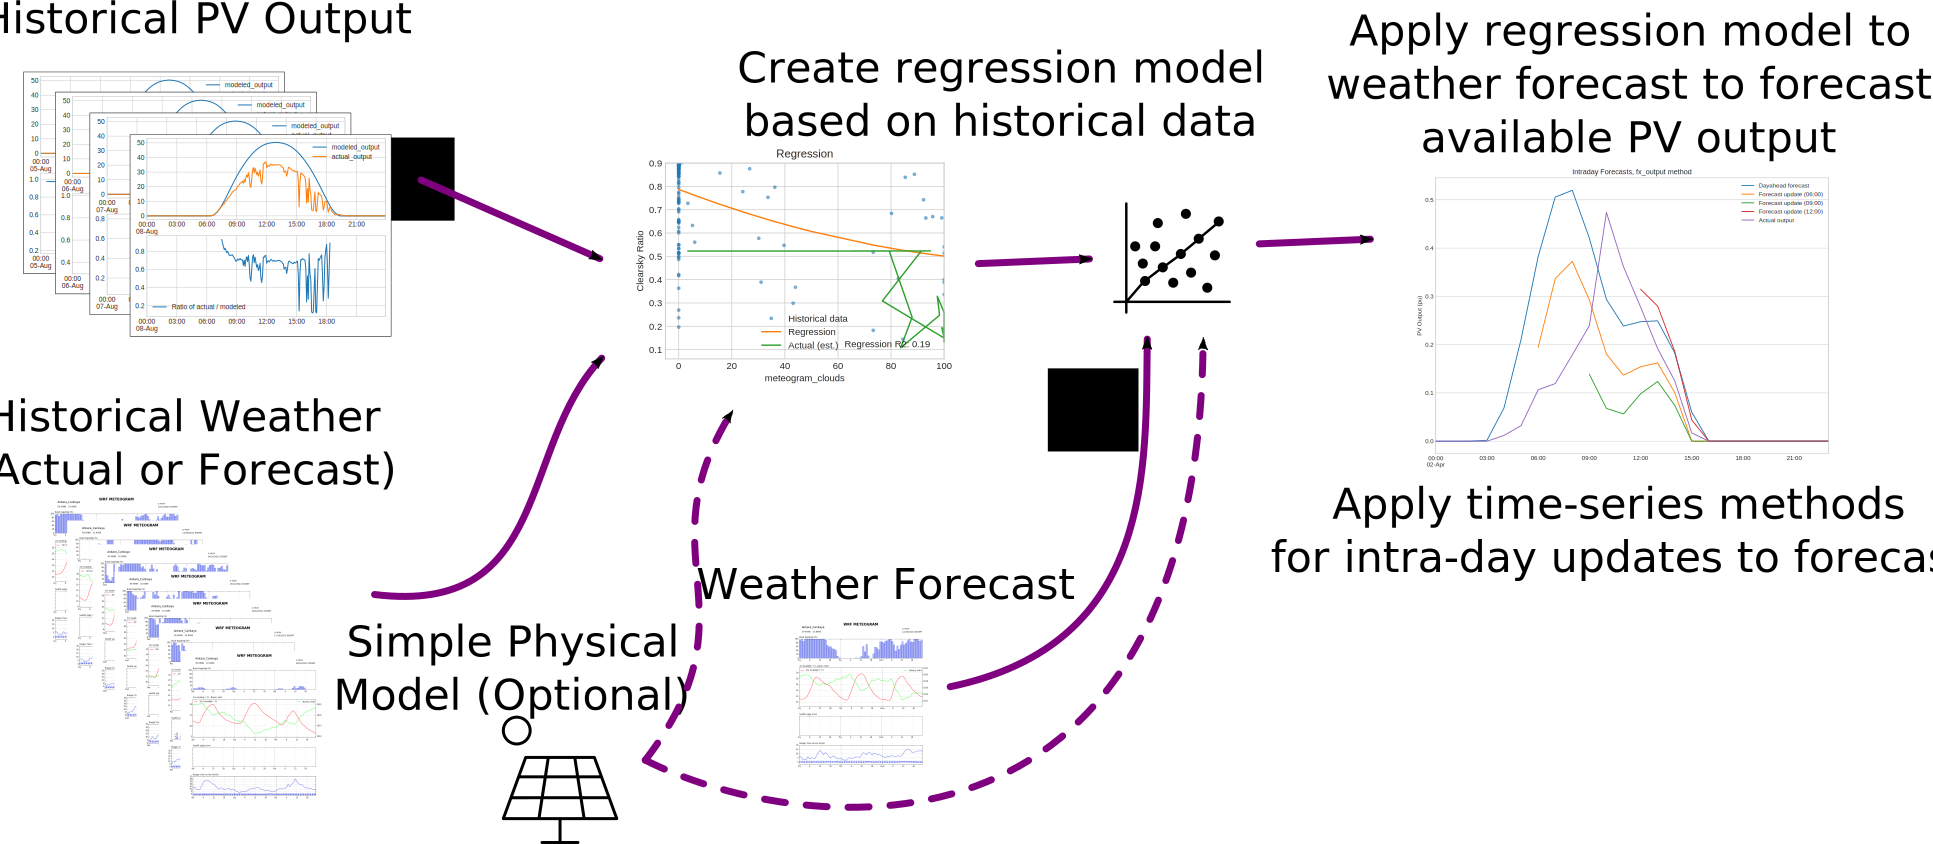
\includegraphics[width=1.0\columnwidth]{PV_forecast_flowchart}
	\caption{Flowchart of Forecasting Method}
	\label{fig:PV_forecast_flowchart}
\end{figure}


\subsection{Day-Ahead Forecasts}
\label{sec:method-day-ahead}

The proposed day-ahead forecasting method combines historical PV output data with historical weather data to infer the relationship between weather and PV output by fitting a simple regression model.

Some pre-processing of the historical data was done prior to  fitting the regression model.
Data from periods of darkness, when output goes to small or negative values, were removed.
This also removed periods when the PV array was covered with snow.

How the regression model was applied depends on the weather data that was used.
If the weather data used represented the incoming solar energy, then the regression was done directly between the weather data and PV output.
Weather data utilized of this type was the global horizontal irradiance (ghi).

On the other hand, weather data that represented the attenuation of incoming solar energy was regressed against the clear-sky ratio for PV output.
Two methods were developed for calculating the clear-sky ratio.
The first method was to roughly model the PV array using data for its geographic position and orientation to obtain modeled clear-sky output.
The second method was to estimate the maximum possible output at each time of day by calculating the maximum observed PV output for each time of day in the historical data window.
This second method had the advantage of not requiring any modeling information about the PV array.
It had the further advantage of naturally incorporating effects of shading of the array during parts of the day due to obstructions.
Since the data set used for this analysis did not include any shading of the array, this last benefit could not be assessed in comparison to other methods.

The formula used to calculate the clear-sky ratio is shown in \cref{eqn:clear-sky-ratio},
where $r_{cs}$ is the clear-sky ratio, $P_{out}$ is the PV output, and $P_{cs}$ is the clear-sky PV output.
In order to provide numerical stability of the clear-sky ratio for periods when the clear-sky output is small, the parameters $\epsilon$ and $r_\epsilon$ were incorporated so that as $P_{cs}$ goes to zero, the clear-sky ratio $r_{cs}$ will approach $r_\epsilon$.

\begin{equation}
	\label{eqn:clear-sky-ratio}
	r_{cs} = \frac{P_{out} + r_\epsilon \epsilon}{P_{cs} + \epsilon}
\end{equation}

The regression model was then fit to the transformed data.
A second-degree polynomial model was used in the case of ghi weather forecasts as well as the case of cloudiness weather forecasts.
The fit model was then applied to the weather forecast data available for the forecast period.
If applicable, the resulting forecast was then converted from a forecast clear-sky ratio back to PV output.

\subsection{Intra-day Updates}
\label{sec:method-intraday}

Based on the assumption that updated weather forecasts are in general not obtained throughout the day, the current-day PV output forecast was updated using time-series techniques. Several approaches to intra-day updates were investigated as described in the following paragraphs.

\textit{AR(2) on actual output with exogenous variable:}
An auto-regressive time series model with two lags was applied to the actual clear-sky output ratio with the day-ahead clear-sky output forecast included in the model as an exogenous variable.

\textit{SARIMAX:}
A seasonal auto-regressive integrated moving average model was applied to the actual PV power output with day-ahead output power forecast included in the model as an exogenous variable.
This model is characterized by parameters for the number of lags, order of differencing, and order of the moving average, for both the trend and seasonal components.
A variety of parameter combinations was tested against the data, and the best performing model was with AR(1) and MA(2), with the day-ahead PV output power forecast as an exogenous variable, and with no differencing or seasonal components included.

\textit{AR(2) on residual of PV output:}
An auto-regressive time series model with two lags was applied to the residual between actual PV output and the day-ahead forecast PV output. The forecast output of the model was then added as a correction term to the day-ahead PV output forecast for the intra-day period.

\textit{AR(2) on residual of clear-sky ratio:}
An auto-regressive time series model with two lags was applied to the residual between the actual clear-sky ratio and the day-ahead forecast clear-sky ratio. The forecast output of the model was then added as a correction term to the day-ahead clear-sky ratio forecast for the intra-day period.

\textit{Scaling:}
The day-ahead forecast for the rest of the day was scaled using the ratio between the actual output in the previous period and the day-ahead forecast for the previous period.



\section{Data Sources}
\label{sec:data-source}

The PV time series used for this analysis was the recorded output power of the rooftop PV array on the METU EEE Department machinery building in Ankara, Turkey.
Recordings were obtained by downloading them from the logger integrated with the inverter for the PV array.
Logged data was recorded at approximately five-minute intervals.
For the forecasting method, the logged data was aligned to exact five-minute intervals even with the hour using linear interpolation and then aggregated to hourly intervals by the mean.
For the operational model, these values were scaled to the rating of the demonstration system.


The weather forecast data used for this analysis was obtained from multiple sources.
Firstly, WRF Meteogram forecasts have been saved from the Turkish Meteorology Directorate (MGM)\cite{MGM_Meteogram}.
Since the MGM meteograms are available as a image rather than as structured data, code was developed to extract data from the plots in the meteogram and output it in csv format\cite{MeteogramExtractGithubRepo}.
Secondly, forecasts were obtained from the SolCast PV-focused weather service\cite{Solcast}.
SolCast weather forecasts include both a cloudiness forecast as well as an irradiance (ghi) forecast along with many other forecast quantities.
SolCast data is provided using an API, so no special data extraction or conversion was needed.

% OpenWeather weather service\cite{OpenWeather} was downloaded but currently is not being used.

\section{Implementation}
\label{sec:implementation}

The forecasting code was implemented using the Python programming language\cite{Python3}.
The Pandas\cite{Pandas} data analysis library and NumPy\cite{NumPy} were used for data manipulation.
Scikit-learn\cite{scikit-learn} was used for fitting the regression model and generating predictions from it.
Statsmodels\cite{statsmodels} was used for fitting time-series auto-regressive models and generating predictions.
Plots were generated using Matplotlib\cite{Matplotlib}.
The optimization and simulation implementation was previously described in \cite{Brown2022}.
Full implementation details can be obtained by examining the source code released on GitHub\cite{ELECO2023GithubRepo} and CodeOcean\cite{ELECO2023CodeOceanRepo}.

\section{Results}
\label{sec:results}

Results will be presented in this section. Plots! Tables! Yay!




\section{Conclusion}
\label{sec:conclusion}

This is the conclusion section. It should be all new and focus on the additional forecasting work to do.

%\clearpage

\section{Acknowledgments}
This work is supported by the Scientific and Technological
Research Council of Turkey (TUBITAK) under grant number
119N313.

\section{References}

% trigger a \newpage just before the given reference
% number - used to balance the columns on the last page
% adjust value as needed - may need to be readjusted if
% the document is modified later
%\IEEEtriggeratref{8}
% The "triggered" command can be changed if desired:
%\IEEEtriggercmd{\enlargethispage{-5in}}

% Enable to reduce spacing between bibitems (source: https://tex.stackexchange.com/a/25774)
% \def\IEEEbibitemsep{0pt plus .5pt}

% argument is your BibTeX string definitions and bibliography database(s)
\bibliography{IEEEabrv,biblio}
% Manually include bibliography for the final version
%% !TeX spellcheck = en-US
% !TeX encoding = utf8
% !TeX program = pdflatex
% !BIB program = bibtex
% -*- coding:utf-8 mod:LaTeX -*-

% To set up:
% aptitude install texlive-publishers texlive-lang-european texlive-latex-extra

% PBROWN: Use this to suppress the warning when including multiple matplotlib PDF plots on the same page
\pdfsuppresswarningpagegroup=1

\RequirePackage{fix-cm}

%cmap has to be loaded before any font package (such as newtxmath)
\RequirePackage{cmap}

% Found eleco2013 code in ELECO 2017 conference archive

\documentclass[9pt]{extarticle}
\usepackage{eleco}

\usepackage{orcidlink}

\usepackage[T1]{fontenc}
\usepackage[utf8]{inputenc} %support umlauts in the input

\usepackage{graphicx}

%\usepackage[inkscapelatex=false]{svg}

%Set English as language and allow to write hyphenated"=words
% For Turkish, on Ubuntu aptitude install texlive-lang-european
%\usepackage[english]{babel}
% If using Turkish, also set option shorthands=off
%Hint by http://tex.stackexchange.com/a/321066/9075 -> enable "= as dashes
%\addto\extrasenglish{\languageshorthands{ngerman}\useshorthands{"}}

% backticks (`) are rendered as such in verbatim environment. See https://tex.stackexchange.com/a/341057/9075 for details.
%\usepackage{upquote}

%for easy quotations: \enquote{text}
\usepackage{csquotes}

%enable margin kerning
\RequirePackage{iftex}
\ifPDFTeX
  \RequirePackage[%
    final,%
    expansion=alltext,%
    protrusion=alltext-nott]{microtype}%
\else
  \RequirePackage[%
    final,%
    protrusion=alltext-nott]{microtype}%
\fi%
% \texttt{test -- test} keeps the "--" as "--" (and does not convert it to an en dash)
%\DisableLigatures{encoding = T1, family = tt* }

%tweak \url{...}
\usepackage{url}
%\urlstyle{same}
%improve wrapping of URLs - hint by http://tex.stackexchange.com/a/10419/9075
\makeatletter
\g@addto@macro{\UrlBreaks}{\UrlOrds}
\makeatother
%nicer // - solution by http://tex.stackexchange.com/a/98470/9075
%DO NOT ACTIVATE -> prevents line breaks
%\makeatletter
%\def\Url@twoslashes{\mathchar`\/\@ifnextchar/{\kern-.2em}{}}
%\g@addto@macro\UrlSpecials{\do\/{\Url@twoslashes}}
%\makeatother

% Diagonal lines in a table - http://tex.stackexchange.com/questions/17745/diagonal-lines-in-table-cell
% Slashbox is not available in texlive (due to licensing) and also gives bad results. This, we use diagbox
%\usepackage{diagbox}

\usepackage{booktabs}
\usepackage{multirow}  % If needed for any  multi-row table cells

% Required for package pdfcomment later
\usepackage{xcolor}

% For listings
%\usepackage{listings}
%\lstset{%
%  basicstyle=\ttfamily,%
%  columns=fixed,%
%  basewidth=.5em,%
%  xleftmargin=0.5cm,%
%  captionpos=b}%

% Enable nice comments
\usepackage[final]{pdfcomment}
%
% color={0.045 0.278 0.643}  % Blue
% color={0.234 0.867 0.211 % Light green
\newcommand{\commentontext}[2]{\colorbox{yellow!60}{#1}\pdfcomment[color={0.234 0.867 0.211},hoffset=-6pt,voffset=10pt,opacity=0.5]{#2}}
\newcommand{\commentatside}[1]{\pdfcomment[color=yellow,icon=Note]{#1}}
%
% Compatibility with packages todo, easy-todo, todonotes
\newcommand{\todo}[1]{\commentatside{#1}}
% Compatiblity with package fixmetodonotes
\newcommand{\TODO}[1]{\commentatside{#1}}

% Bibliography enhancements
%  - enable \cite[prenote][]{ref}
%  - enable \cite{ref1,ref2}
% Alternative: \usepackage{cite}, which enables \cite{ref1, ref2} only (otherwise: Error message: "White space in argument")
%
% Doc: http://texdoc.net/natbib

% normal IEEE
%\usepackage[%
%	square,        % for square brackets
%	comma,         % use commas as separators
%	numbers,       % for numerical citations;
%	%sort           % orders multiple citations into the sequence in which they appear in the list of references;
%	sort&compress % as sort but in addition multiple numerical citations
%	               % are compressed if possible (as 3-6, 15);
%]{natbib}
% Same fontsize as without natbib
%\renewcommand{\bibfont}{\normalfont\footnotesize}
% Using cite package instead
\usepackage{cite}

% Enable hyperlinked author names in the case of \citet
% Source: https://tex.stackexchange.com/a/76075/9075
%\usepackage{etoolbox}
%\makeatletter
%\patchcmd{\NAT@test}{\else \NAT@nm}{\else \NAT@hyper@{\NAT@nm}}{}{}
%\makeatother

% Enable that parameters of \cref{}, \ref{}, \cite{}, ... are linked so that a reader can click on the number an jump to the target in the document
\usepackage{hyperref}
% Enable hyperref without colors and without bookmarks
\hypersetup{hidelinks,
  colorlinks=true,
  allcolors=black,
  pdfstartview=Fit,
  breaklinks=true}
%
% Enable correct jumping to figures when referencing
\usepackage[all]{hypcap}

%\renewcommand{\figurename}{Fig.}

%enable \cref{...} and \Cref{...} instead of \ref: Type of reference included in the link
\usepackage[capitalise,nameinlink]{cleveref}
% The following are to comply with the IEEE style guide.
\crefformat{equation}{#2(#1)#3}
\Crefformat{equation}{#2Equation (#1)#3}
\crefname{figure}{Fig.}{Figs.}

%Following definitions are outside of IfPackageLoaded; inside, they are not visible
%
%Intermediate solution for hyperlinked refs. See https://tex.stackexchange.com/q/132420/9075 for more information.
%\newcommand{\Vlabel}[1]{\label[line]{#1}\hypertarget{#1}{}}
%\newcommand{\lref}[1]{\hyperlink{#1}{\FancyVerbLineautorefname~\ref*{#1}}}
%
%\newenvironment{listing}[1][htbp!]{\begin{figure}[#1]}{\end{figure}}
%\newcounter{listing}

%\usepackage{xspace}
%\newcommand{\eg}{e.\,g.\xspace}
%\newcommand{\ie}{i.\,e.\xspace}
\newcommand{\eg}{e.\,g.,\ }
\newcommand{\ie}{i.\,e.,\ }

%%introduce \powerset - hint by http://matheplanet.com/matheplanet/nuke/html/viewtopic.php?topic=136492&post_id=997377
%\DeclareFontFamily{U}{MnSymbolC}{}
%\DeclareSymbolFont{MnSyC}{U}{MnSymbolC}{m}{n}
%\DeclareFontShape{U}{MnSymbolC}{m}{n}{
%  <-6>    MnSymbolC5
%  <6-7>   MnSymbolC6
%  <7-8>   MnSymbolC7
%  <8-9>   MnSymbolC8
%  <9-10>  MnSymbolC9
%  <10-12> MnSymbolC10
%  <12->   MnSymbolC12%
%}{}
%\DeclareMathSymbol{\powerset}{\mathord}{MnSyC}{180}

% *** SUBFIGURE PACKAGES ***
%\usepackage[caption=false,font=footnotesize]{subfig}

%\usepackage{stfloats}



% correct bad hyphenation here
\hyphenation{op-tical net-works semi-conduc-tor}

\graphicspath{{./figs/}}

% Paper-specific packages that I have added:
\usepackage{siunitx}  % For units with \SI
\usepackage{threeparttable}  % For tablenotes
\usepackage{placeins}  % For \FloatBarrier
\usepackage{xfrac}  % For \sfrac
%\usepackage{orcidlink}  % For orcid link
\DeclareMathOperator{\logicand}{and}
\DeclareMathOperator{\logicor}{or}


%\bibliographystyle{chicago}   % For drafts only, to make it easier to see which references have been used.
%\bibliographystyle{IEEEtran} % IEEEtranN is the natbib compatible bst file
%\usepackage{showkeys}          % For drafts only


\begin{document}
%\IEEEoverridecommandlockouts
\bstctlcite{IEEEexample:BSTcontrol}

\title{Lightweight Photovoltaic Forecasting Method for Agricultural Microgrids}

\author{%
  \IEEEauthorblockN{Paul D. Brown}%\textsuperscript{\orcidlink{0000-0001-5753-0449}}}%
  \IEEEauthorblockA{Department of Electrical and Electronics Engineering\\
  	Middle East Technical University\\
  	Ankara, Turkey\\
  	ORCID: 0000-0001-5753-0449}
\and
  \IEEEauthorblockN{Murat Göl}%\textsuperscript{\orcidlink{0000-0002-2523-1169}}}%
  %\orcidlink{0000-0001-5753-0449}
  \IEEEauthorblockA{Department of Electrical and Electronics Engineering\\
    Middle East Technical University\\
	Ankara, Turkey\\
	ORCID: 0000-0002-2523-1169}
}

% No paper headers for conference
%\markboth{ISGT Europe, October 2023}%
%{{Brown}: Lightweight Photovoltaic Forecasting Method for Agricultural Microgrid}

% make the title area
\maketitle
\begin{abstract}
  % Abstract_should_be_150_to_200_words.
A lightweight forecasting method was developed for day-ahead (12 to 72-hours) and intra-day forecasting of photovoltaic (PV) array power output for use with energy management of agricultural microgrids.
The proposed method allows the PV output to be forecast without requiring extensive computing resources or high-bandwidth communication channel to the PV site.
The proposed day-ahead forecasting method combines historical PV output data with historical weather data to infer the relationship between weather and PV output by fitting a simple regression model.
Based on the assumption that updated weather forecasts are in general not obtained throughout the day, the current-day PV output forecast was updated using time-series techniques.
The proposed forecasting methods were applied to a dataset of rooftop PV output
and compared to reference persistence forecasts.
The method was demonstrated by using the forecasts in the optimized operation of an agricultural microgrid
and simulating with actual PV output.
\end{abstract}

\section{Introduction}
\label{sec:intro}

Over recent decades, many factors have driven significant changes in the electrical power industry,
including climate change,
the growing use of renewable energy resources,
and ongoing rural electrification.
For agricultural consumers, electrification enables increased yields and economic development.
Ref. \cite{Mandelli2016} reviews technology and applications for off-grid systems for rural electrification.

For agricultural applications, photovoltaic (PV) energy is generally well aligned with water needs\cite{Aliyu2018}.
Ref. \cite{Aliyu2018} reviews numerous solar-powered water pumping applications around the world while \cite{Muhsen2017} reviews the PV and water pumping modeling, design, and control approaches in the literature.

One of the barriers to efficient use of PV energy in the grid and in micro-grids
is the difficulty of accurately predicting future energy availability.
As reviewed in \cite{Antonanzas2016}, many techniques have been developed for forecasting PV energy over various time horizons.
The authors of this paper have been working on techniques for optimal energy planning for agricultural microgrids.
For operational optimization, an effective day-ahead PV forecasting method was needed.
In recent years, LSTM-based neural networks have emerged as the state-of-the art
for day-ahead PV energy forecasting
\cite{Kuo2022,Aslam2021,Liu2021}.

As promising as deep learning networks are for day-ahead forecasting,
they have the drawback of requiring 
a lot of historical data\cite{Aillaud2020} and significant computational resources for training.
Agricultural microgrids, on the other hand, are often implemented in locations where communication infrastructure is weak
and bandwidth and/or availability are limited.
To cope with these conditions, the authors developed methods for day-ahead PV forecasting with a design goal to be ``lightweight'', that is to require minimal weather forecast data, site-specific modeling data, historical generation data, and computational resources.
The target computing platform for the developed method is a single-board computer such as the Raspberry Pi or similar.


The literature survey will be part of the introduction.







% Make sure any figures start AFTER the introduction and don't float above it.
\FloatBarrier

\section{Proposed Method}
\label{sec:proposed-method}

The proposed method utilizes meteorological forecast data such as forecast cloudiness or forecast irradiance to forecast the PV system output for the upcoming 12 to 72 hours, which called the ``day-ahead forecast''.
It is assumed that these meteorological forecasts will be updated once or at most a few times per day.
Throughout the day, the current day's PV output forecast is updated by applying one of several available time-series forecasting techniques.
A high-level diagram of the proposed forecast method is shown in \cref{fig:PV_forecast_flowchart}.

\begin{figure}[t]
	\centering
	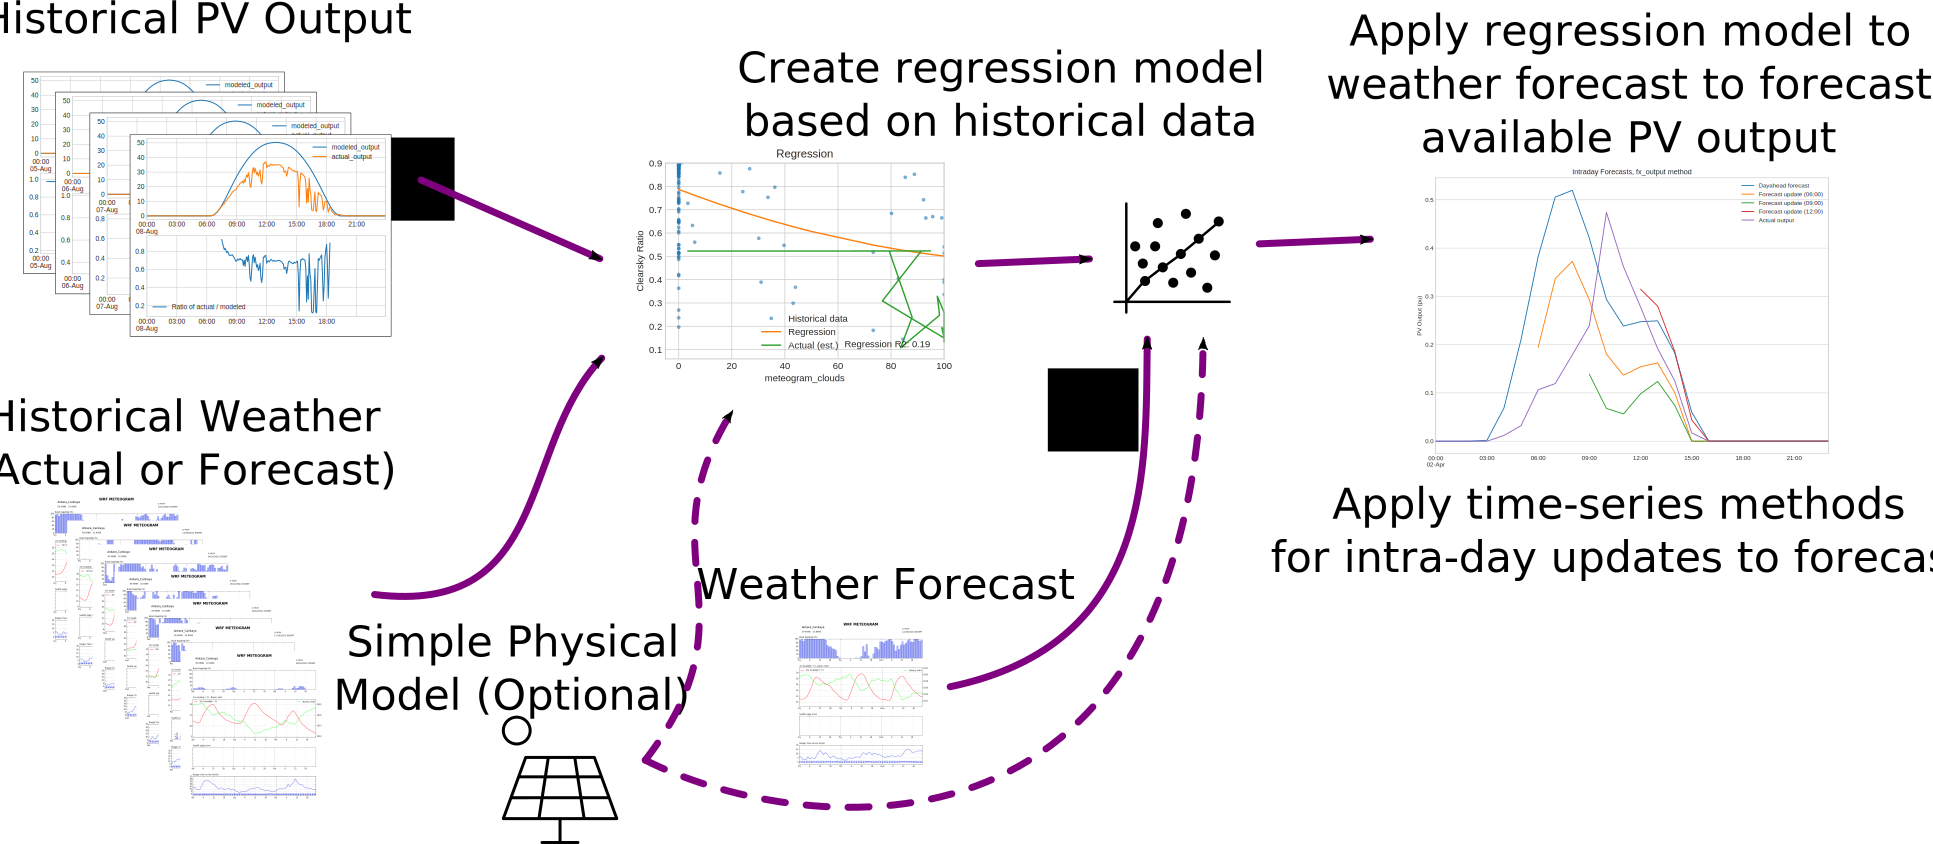
\includegraphics[width=1.0\columnwidth]{PV_forecast_flowchart}
	\caption{Flowchart of Forecasting Method}
	\label{fig:PV_forecast_flowchart}
\end{figure}


\subsection{Day-Ahead Forecasts}
\label{sec:method-day-ahead}

The proposed day-ahead forecasting method combines historical PV output data with historical weather data to infer the relationship between weather and PV output by fitting a simple regression model.

Some pre-processing of the historical data was done prior to  fitting the regression model.
Data from periods of darkness, when output goes to small or negative values, were removed.
This also removed periods when the PV array was covered with snow.

How the regression model was applied depends on the weather data that was used.
If the weather data used represented the incoming solar energy, then the regression was done directly between the weather data and PV output.
Weather data utilized of this type was the global horizontal irradiance (ghi).

On the other hand, weather data that represented the attenuation of incoming solar energy was regressed against the clear-sky ratio for PV output.
Two methods were developed for calculating the clear-sky ratio.
The first method was to roughly model the PV array using data for its geographic position and orientation to obtain modeled clear-sky output.
The second method was to estimate the maximum possible output at each time of day by calculating the maximum observed PV output for each time of day in the historical data window.
This second method had the advantage of not requiring any modeling information about the PV array.
It had the further advantage of naturally incorporating effects of shading of the array during parts of the day due to obstructions.
Since the data set used for this analysis did not include any shading of the array, this last benefit could not be assessed in comparison to other methods.

The formula used to calculate the clear-sky ratio is shown in \cref{eqn:clear-sky-ratio},
where $r_{cs}$ is the clear-sky ratio, $P_{out}$ is the PV output, and $P_{cs}$ is the clear-sky PV output.
In order to provide numerical stability of the clear-sky ratio for periods when the clear-sky output is small, the parameters $\epsilon$ and $r_\epsilon$ were incorporated so that as $P_{cs}$ goes to zero, the clear-sky ratio $r_{cs}$ will approach $r_\epsilon$.

\begin{equation}
	\label{eqn:clear-sky-ratio}
	r_{cs} = \frac{P_{out} + r_\epsilon \epsilon}{P_{cs} + \epsilon}
\end{equation}

The regression model was then fit to the transformed data.
A second-degree polynomial model was used in the case of ghi weather forecasts as well as the case of cloudiness weather forecasts.
The fit model was then applied to the weather forecast data available for the forecast period.
If applicable, the resulting forecast was then converted from a forecast clear-sky ratio back to PV output.

\subsection{Intra-day Updates}
\label{sec:method-intraday}

Based on the assumption that updated weather forecasts are in general not obtained throughout the day, the current-day PV output forecast was updated using time-series techniques. Several approaches to intra-day updates were investigated as described in the following paragraphs.

\textit{AR(2) on actual output with exogenous variable:}
An auto-regressive time series model with two lags was applied to the actual clear-sky output ratio with the day-ahead clear-sky output forecast included in the model as an exogenous variable.

\textit{SARIMAX:}
A seasonal auto-regressive integrated moving average model was applied to the actual PV power output with day-ahead output power forecast included in the model as an exogenous variable.
This model is characterized by parameters for the number of lags, order of differencing, and order of the moving average, for both the trend and seasonal components.
A variety of parameter combinations was tested against the data, and the best performing model was with AR(1) and MA(2), with the day-ahead PV output power forecast as an exogenous variable, and with no differencing or seasonal components included.

\textit{AR(2) on residual of PV output:}
An auto-regressive time series model with two lags was applied to the residual between actual PV output and the day-ahead forecast PV output. The forecast output of the model was then added as a correction term to the day-ahead PV output forecast for the intra-day period.

\textit{AR(2) on residual of clear-sky ratio:}
An auto-regressive time series model with two lags was applied to the residual between the actual clear-sky ratio and the day-ahead forecast clear-sky ratio. The forecast output of the model was then added as a correction term to the day-ahead clear-sky ratio forecast for the intra-day period.

\textit{Scaling:}
The day-ahead forecast for the rest of the day was scaled using the ratio between the actual output in the previous period and the day-ahead forecast for the previous period.



\section{Data Sources}
\label{sec:data-source}

The PV time series used for this analysis was the recorded output power of the rooftop PV array on the METU EEE Department machinery building in Ankara, Turkey.
Recordings were obtained by downloading them from the logger integrated with the inverter for the PV array.
Logged data was recorded at approximately five-minute intervals.
For the forecasting method, the logged data was aligned to exact five-minute intervals even with the hour using linear interpolation and then aggregated to hourly intervals by the mean.
For the operational model, these values were scaled to the rating of the demonstration system.


The weather forecast data used for this analysis was obtained from multiple sources.
Firstly, WRF Meteogram forecasts have been saved from the Turkish Meteorology Directorate (MGM)\cite{MGM_Meteogram}.
Since the MGM meteograms are available as a image rather than as structured data, code was developed to extract data from the plots in the meteogram and output it in csv format\cite{MeteogramExtractGithubRepo}.
Secondly, forecasts were obtained from the SolCast PV-focused weather service\cite{Solcast}.
SolCast weather forecasts include both a cloudiness forecast as well as an irradiance (ghi) forecast along with many other forecast quantities.
SolCast data is provided using an API, so no special data extraction or conversion was needed.

% OpenWeather weather service\cite{OpenWeather} was downloaded but currently is not being used.

\section{Implementation}
\label{sec:implementation}

The forecasting code was implemented using the Python programming language\cite{Python3}.
The Pandas\cite{Pandas} data analysis library and NumPy\cite{NumPy} were used for data manipulation.
Scikit-learn\cite{scikit-learn} was used for fitting the regression model and generating predictions from it.
Statsmodels\cite{statsmodels} was used for fitting time-series auto-regressive models and generating predictions.
Plots were generated using Matplotlib\cite{Matplotlib}.
The optimization and simulation implementation was previously described in \cite{Brown2022}.
Full implementation details can be obtained by examining the source code released on GitHub\cite{ELECO2023GithubRepo} and CodeOcean\cite{ELECO2023CodeOceanRepo}.

\section{Results}
\label{sec:results}

Results will be presented in this section. Plots! Tables! Yay!




\section{Conclusion}
\label{sec:conclusion}

This is the conclusion section. It should be all new and focus on the additional forecasting work to do.

%\clearpage

\section{Acknowledgments}
This work is supported by the Scientific and Technological
Research Council of Turkey (TUBITAK) under grant number
119N313.

\section{References}

% trigger a \newpage just before the given reference
% number - used to balance the columns on the last page
% adjust value as needed - may need to be readjusted if
% the document is modified later
%\IEEEtriggeratref{8}
% The "triggered" command can be changed if desired:
%\IEEEtriggercmd{\enlargethispage{-5in}}

% Enable to reduce spacing between bibitems (source: https://tex.stackexchange.com/a/25774)
% \def\IEEEbibitemsep{0pt plus .5pt}

% argument is your BibTeX string definitions and bibliography database(s)
\bibliography{IEEEabrv,biblio}
% Manually include bibliography for the final version
%% !TeX spellcheck = en-US
% !TeX encoding = utf8
% !TeX program = pdflatex
% !BIB program = bibtex
% -*- coding:utf-8 mod:LaTeX -*-

% To set up:
% aptitude install texlive-publishers texlive-lang-european texlive-latex-extra

% PBROWN: Use this to suppress the warning when including multiple matplotlib PDF plots on the same page
\pdfsuppresswarningpagegroup=1

\RequirePackage{fix-cm}

%cmap has to be loaded before any font package (such as newtxmath)
\RequirePackage{cmap}

% Found eleco2013 code in ELECO 2017 conference archive

\documentclass[9pt]{extarticle}
\usepackage{eleco}

\usepackage{orcidlink}

\usepackage[T1]{fontenc}
\usepackage[utf8]{inputenc} %support umlauts in the input

\usepackage{graphicx}

%\usepackage[inkscapelatex=false]{svg}

%Set English as language and allow to write hyphenated"=words
% For Turkish, on Ubuntu aptitude install texlive-lang-european
%\usepackage[english]{babel}
% If using Turkish, also set option shorthands=off
%Hint by http://tex.stackexchange.com/a/321066/9075 -> enable "= as dashes
%\addto\extrasenglish{\languageshorthands{ngerman}\useshorthands{"}}

% backticks (`) are rendered as such in verbatim environment. See https://tex.stackexchange.com/a/341057/9075 for details.
%\usepackage{upquote}

%for easy quotations: \enquote{text}
\usepackage{csquotes}

%enable margin kerning
\RequirePackage{iftex}
\ifPDFTeX
  \RequirePackage[%
    final,%
    expansion=alltext,%
    protrusion=alltext-nott]{microtype}%
\else
  \RequirePackage[%
    final,%
    protrusion=alltext-nott]{microtype}%
\fi%
% \texttt{test -- test} keeps the "--" as "--" (and does not convert it to an en dash)
%\DisableLigatures{encoding = T1, family = tt* }

%tweak \url{...}
\usepackage{url}
%\urlstyle{same}
%improve wrapping of URLs - hint by http://tex.stackexchange.com/a/10419/9075
\makeatletter
\g@addto@macro{\UrlBreaks}{\UrlOrds}
\makeatother
%nicer // - solution by http://tex.stackexchange.com/a/98470/9075
%DO NOT ACTIVATE -> prevents line breaks
%\makeatletter
%\def\Url@twoslashes{\mathchar`\/\@ifnextchar/{\kern-.2em}{}}
%\g@addto@macro\UrlSpecials{\do\/{\Url@twoslashes}}
%\makeatother

% Diagonal lines in a table - http://tex.stackexchange.com/questions/17745/diagonal-lines-in-table-cell
% Slashbox is not available in texlive (due to licensing) and also gives bad results. This, we use diagbox
%\usepackage{diagbox}

\usepackage{booktabs}
\usepackage{multirow}  % If needed for any  multi-row table cells

% Required for package pdfcomment later
\usepackage{xcolor}

% For listings
%\usepackage{listings}
%\lstset{%
%  basicstyle=\ttfamily,%
%  columns=fixed,%
%  basewidth=.5em,%
%  xleftmargin=0.5cm,%
%  captionpos=b}%

% Enable nice comments
\usepackage[final]{pdfcomment}
%
% color={0.045 0.278 0.643}  % Blue
% color={0.234 0.867 0.211 % Light green
\newcommand{\commentontext}[2]{\colorbox{yellow!60}{#1}\pdfcomment[color={0.234 0.867 0.211},hoffset=-6pt,voffset=10pt,opacity=0.5]{#2}}
\newcommand{\commentatside}[1]{\pdfcomment[color=yellow,icon=Note]{#1}}
%
% Compatibility with packages todo, easy-todo, todonotes
\newcommand{\todo}[1]{\commentatside{#1}}
% Compatiblity with package fixmetodonotes
\newcommand{\TODO}[1]{\commentatside{#1}}

% Bibliography enhancements
%  - enable \cite[prenote][]{ref}
%  - enable \cite{ref1,ref2}
% Alternative: \usepackage{cite}, which enables \cite{ref1, ref2} only (otherwise: Error message: "White space in argument")
%
% Doc: http://texdoc.net/natbib

% normal IEEE
%\usepackage[%
%	square,        % for square brackets
%	comma,         % use commas as separators
%	numbers,       % for numerical citations;
%	%sort           % orders multiple citations into the sequence in which they appear in the list of references;
%	sort&compress % as sort but in addition multiple numerical citations
%	               % are compressed if possible (as 3-6, 15);
%]{natbib}
% Same fontsize as without natbib
%\renewcommand{\bibfont}{\normalfont\footnotesize}
% Using cite package instead
\usepackage{cite}

% Enable hyperlinked author names in the case of \citet
% Source: https://tex.stackexchange.com/a/76075/9075
%\usepackage{etoolbox}
%\makeatletter
%\patchcmd{\NAT@test}{\else \NAT@nm}{\else \NAT@hyper@{\NAT@nm}}{}{}
%\makeatother

% Enable that parameters of \cref{}, \ref{}, \cite{}, ... are linked so that a reader can click on the number an jump to the target in the document
\usepackage{hyperref}
% Enable hyperref without colors and without bookmarks
\hypersetup{hidelinks,
  colorlinks=true,
  allcolors=black,
  pdfstartview=Fit,
  breaklinks=true}
%
% Enable correct jumping to figures when referencing
\usepackage[all]{hypcap}

%\renewcommand{\figurename}{Fig.}

%enable \cref{...} and \Cref{...} instead of \ref: Type of reference included in the link
\usepackage[capitalise,nameinlink]{cleveref}
% The following are to comply with the IEEE style guide.
\crefformat{equation}{#2(#1)#3}
\Crefformat{equation}{#2Equation (#1)#3}
\crefname{figure}{Fig.}{Figs.}

%Following definitions are outside of IfPackageLoaded; inside, they are not visible
%
%Intermediate solution for hyperlinked refs. See https://tex.stackexchange.com/q/132420/9075 for more information.
%\newcommand{\Vlabel}[1]{\label[line]{#1}\hypertarget{#1}{}}
%\newcommand{\lref}[1]{\hyperlink{#1}{\FancyVerbLineautorefname~\ref*{#1}}}
%
%\newenvironment{listing}[1][htbp!]{\begin{figure}[#1]}{\end{figure}}
%\newcounter{listing}

%\usepackage{xspace}
%\newcommand{\eg}{e.\,g.\xspace}
%\newcommand{\ie}{i.\,e.\xspace}
\newcommand{\eg}{e.\,g.,\ }
\newcommand{\ie}{i.\,e.,\ }

%%introduce \powerset - hint by http://matheplanet.com/matheplanet/nuke/html/viewtopic.php?topic=136492&post_id=997377
%\DeclareFontFamily{U}{MnSymbolC}{}
%\DeclareSymbolFont{MnSyC}{U}{MnSymbolC}{m}{n}
%\DeclareFontShape{U}{MnSymbolC}{m}{n}{
%  <-6>    MnSymbolC5
%  <6-7>   MnSymbolC6
%  <7-8>   MnSymbolC7
%  <8-9>   MnSymbolC8
%  <9-10>  MnSymbolC9
%  <10-12> MnSymbolC10
%  <12->   MnSymbolC12%
%}{}
%\DeclareMathSymbol{\powerset}{\mathord}{MnSyC}{180}

% *** SUBFIGURE PACKAGES ***
%\usepackage[caption=false,font=footnotesize]{subfig}

%\usepackage{stfloats}



% correct bad hyphenation here
\hyphenation{op-tical net-works semi-conduc-tor}

\graphicspath{{./figs/}}

% Paper-specific packages that I have added:
\usepackage{siunitx}  % For units with \SI
\usepackage{threeparttable}  % For tablenotes
\usepackage{placeins}  % For \FloatBarrier
\usepackage{xfrac}  % For \sfrac
%\usepackage{orcidlink}  % For orcid link
\DeclareMathOperator{\logicand}{and}
\DeclareMathOperator{\logicor}{or}


%\bibliographystyle{chicago}   % For drafts only, to make it easier to see which references have been used.
%\bibliographystyle{IEEEtran} % IEEEtranN is the natbib compatible bst file
%\usepackage{showkeys}          % For drafts only


\begin{document}
%\IEEEoverridecommandlockouts
\bstctlcite{IEEEexample:BSTcontrol}

\input{title}

% make the title area
\maketitle
\begin{abstract}
  \input{abstract}
\end{abstract}

\input{01_introduction}

\input{02_lit_survey}

% Make sure any figures start AFTER the introduction and don't float above it.
\FloatBarrier

\input{03_proposed_method}

\input{04_data_sources}

\input{05_implementation}

\input{06_results}

\input{99_conclusion}

%\clearpage

\section{Acknowledgments}
This work is supported by the Scientific and Technological
Research Council of Turkey (TUBITAK) under grant number
119N313.

\section{References}

% trigger a \newpage just before the given reference
% number - used to balance the columns on the last page
% adjust value as needed - may need to be readjusted if
% the document is modified later
%\IEEEtriggeratref{8}
% The "triggered" command can be changed if desired:
%\IEEEtriggercmd{\enlargethispage{-5in}}

% Enable to reduce spacing between bibitems (source: https://tex.stackexchange.com/a/25774)
% \def\IEEEbibitemsep{0pt plus .5pt}

% argument is your BibTeX string definitions and bibliography database(s)
\bibliography{IEEEabrv,biblio}
% Manually include bibliography for the final version
%\input{build/Paul_Brown_Paper.bbl}


\end{document}



\end{document}



\end{document}


%\ \\ % empty line after bibliogpraphy and that statement

\begin{IEEEbiography}[{\includegraphics[width=1in,height=1.25in,clip,keepaspectratio]{Photo_Paul}}]{Paul Brown}
	(S’03–M’06)
	received the B.S. in Electrical Engineering from Iowa State University, Ames, in 2004
	and the M.S. in Electrical Engineering from the Faculty of Engineering, University of Porto, Porto, Portugal, in 2006.
	He is currently working toward a Ph.D. in Electrical and Electronics Engineering at Middle East Technical University in Ankara, Turkey, under the supervision of Murat Göl.
	He worked as a consulting electrical engineer for Peak Power Engineering in Golden, Colorado, from 2006-2013.
	He worked as a transmission system protection engineer for Nebraska Public Power District in Columbus, Nebraska, from 2013-2017.
\end{IEEEbiography}

\end{document}
